% ==============================================================================
% TCC - Nome do Aluno
% Capítulo 5 - Testes Computacionais
% ==============================================================================
\chapter{Testes Computacionais}
\label{sec-testes}

\section{Algoritmo de Dijkstra}
\label{sec-dijkstra-experimentos}
Para a realização dos experimentos computacionais são utilizadas instâncias de grafos que representam malhas rodoviárias reais. Todas elas descritas nas tabelas \ref{tbl-dijkstra-instancias} e \ref{tbl-dijkstra-configuracao}, e disponíveis no sítio eletrônico \url{http://www.dis.uniroma1.it/challenge9/download.shtml} (acesso em 28 de janeiro de 2017).

A tabela \ref{tbl-dijkstra-instancias} mostra o nome dos arquivos das instâncias que foram executadas para os testes e suas respectivas descrições dos grafos que representam malhas viárias reais. A tabela \ref{tbl-dijkstra-configuracao} mostra a configuração dos respectivos grafos apresentados na tabela \ref{tbl-dijkstra-instancias}, com seus respectivos número de vértices |V| e número de arestas |E|.
\begin{table}[H]
\caption{Instâncias a serem rodadas pelo algoritmo de Dijkstra em suas três versões.}
\label{tbl-dijkstra-instancias}
\centering
\begin{adjustbox}{max width=\textwidth}
\begin{tabular}{|c|c|}
\hline 
\textbf{Nome Instância} & \textbf{Descrição} \\ 
\hline 
USA-road-d.NY.gr & Representa a malha viária do estado de Nova Iorque, Estados Unidos \\ 
\hline 
USA-road-d.BAY.gr & Representa a malha viária da bahia de São Francisco, Califórnia, Estados Unidos \\ 
\hline 
USA-road-d.COL.gr & Representa a malha viária do estado do Colorado, Estados Unidos \\ 
\hline 
USA-road-d.FLA.gr & Representa a malha viária do estado da Flórida, Estados Unidos \\ 
\hline 
\end{tabular}
\end{adjustbox}
\end{table}

\begin{table}[H]
\caption{Configuração dos grafos correspondentes as malhas viárias descritas na tabela \ref{tbl-dijkstra-instancias}.}
\label{tbl-dijkstra-configuracao}
\centering
\begin{adjustbox}{max width=\textwidth}
\begin{tabular}{|c|c|c|}
\hline 
\textbf{Nome Instância} & \textbf{Número de Vértices |V|} & \textbf{Número de Arestas |E|} \\ 
\hline 
USA-road-d.NY.gr
 & 264.346
 & 733.846
 \\ 
\hline 
USA-road-d.BAY.gr
 & 321.270
 & 800.172
 \\ 
\hline 
USA-road-d.COL.gr
 & 435.666
 & 1.057.066
 \\ 
\hline 
USA-road-d.FLA.gr
 & 1.070.376
 & 2.712.798
 \\ 
\hline 
\end{tabular}
\end{adjustbox} 
\end{table}

\subsection{Resultados obtidos}
\label{sec-dijkstra-experimentos-resultados}
Os resultados dos testes obtidos estão descritos a seguir.

\begin{figure}[H]
\centering
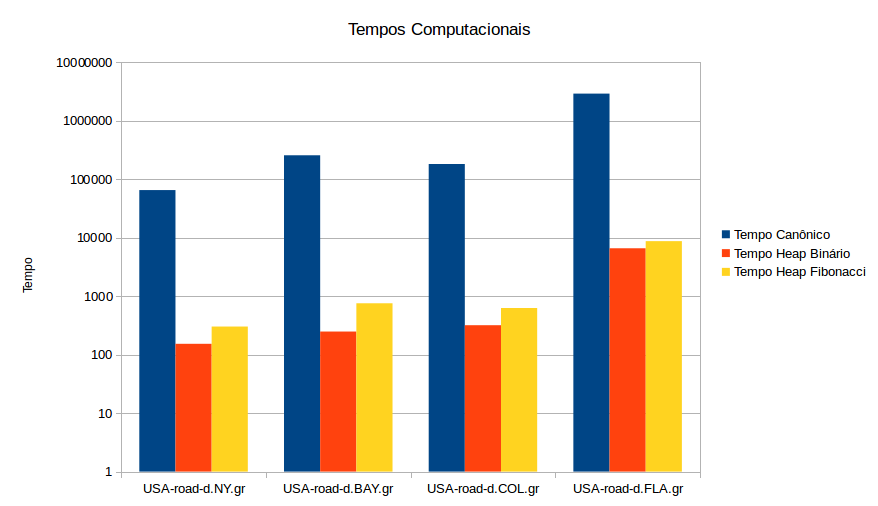
\includegraphics[width=.90\textwidth]{figuras/dijkstra-tempos} 
\caption{Tempos computacionais obtidos pelos Métodos de Dijkstra empregados (tempo em escala logarítmica).}
\label{fig-dijkstra-resultados-tempos}
\end{figure}

\begin{figure}[H]
\centering
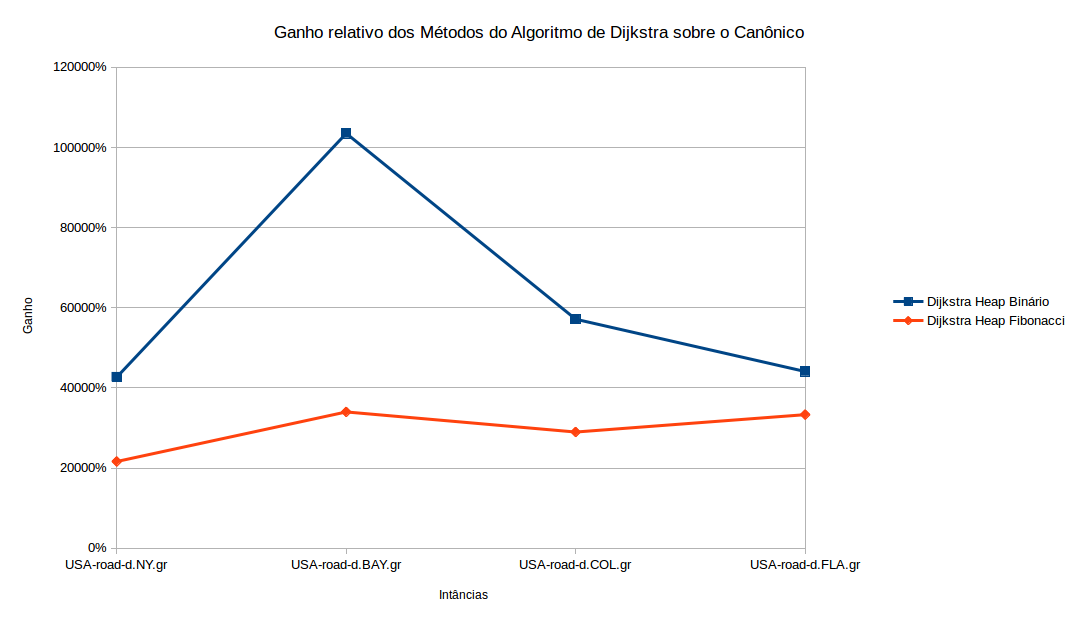
\includegraphics[width=.90\textwidth]{figuras/speed-up-dijkstra} 
\caption{Ganho relativo dos Métodos do Algoritmo de Dijkstra sobre o Canônico.}
\label{fig-dijkstra-resultados-speedup}
\end{figure}


\begin{table}[H]
\caption{Tempos Computacionais obtidos pelo algoritmo de Dijkstra em suas diferentes versões (tempo em milissegundos).}
\label{tbl-dijkstra-resultados-tempos}
\centering
\begin{adjustbox}{max width=\textwidth}
\begin{tabular}{|c|c|c|c|}
\hline
\textbf{Nome Instância} & \textbf{Tempo Canônico} & \textbf{Tempo Heap Binário} & \textbf{Tempo Heap Fibonacci} \\ \hline
USA-road-d.NY.gr        & 65287                   & 153                         & 302                           \\ \hline
USA-road-d.BAY.gr       & 256690                  & 248                         & 755                           \\ \hline
USA-road-d.COL.gr       & 181687                  & 318                         & 627                           \\ \hline
USA-road-d.FLA.gr       & 2909655                 & 6601                        & 8732                          \\ \hline
\end{tabular}
\end{adjustbox}
\end{table}


\begin{table}[H]
\caption{Ganho relativo sobre o Dijkstra Canônico.}
\label{tbl-dijkstra-resultados-speedup}
\centering
\begin{adjustbox}{max width=\textwidth}
\begin{tabular}{|c|c|c|}
\hline
\textbf{Nome Instância} & \textbf{Ganho Heap Binário} & \textbf{Ganho Heap Fibonacci} \\ \hline
USA-road-d.NY.gr        & 42.671\%                       & 21.618\%                         \\ \hline
USA-road-d.BAY.gr       & 103.504\%                      & 33.999\%                         \\ \hline
USA-road-d.COL.gr       & 57.134\%                       & 28.977\%                         \\ \hline
USA-road-d.FLA.gr       & 44.079\%                       & 33.322\%                         \\ \hline
\end{tabular}
\end{adjustbox}
\end{table}

A figura \ref{fig-dijkstra-resultados-tempos} mostra o comparativo entre os tempos computacionais obtidos por cada método em escala logarítmica. A figura \ref{fig-dijkstra-resultados-speedup} mostra o ganho relativo em tempo entre os métodos Dijkstra Heap Binário e Dijkstra Heap de Fibonacci sobre o Dijkstra Canônico. As tabelas \ref{tbl-dijkstra-resultados-tempos} e \ref{tbl-dijkstra-resultados-speedup} mostram os resultados, em números, dos tempos computacionais obtidos e os ganhos relativos sobre o Dijkstra Canônico, respectivamente.

\subsection{Análise dos resultados}
\label{sec-dijkstra-experimentos-analise}
Podemos observar que o Dijkstra Canônico foi executado em um tempo elevado (a instância USA-road-d.FLA.gr por exemplo foi executado em aproximadamente 48 minutos). Já o uso de estrutura de dados impactou consideravelmente no ganho do tempo sendo que o Heap Binário teve um ganho médio de 61.847\% com relação ao Dijkstra Canônico enquanto Dijkstra Heap de Fibonacci teve um ganho médio de 29.479\% (vide tabela \ref{tbl-dijkstra-resultados-speedup}).

Com relação ao resultado obtido pelos métodos do Heap Binário e Heap de Fibonacci, ele é de certo modo inesperado, já que conforme mostrado nas subseções \ref{sec-dijkstra-versoes-heap} e \ref{sec-dijkstra-versoes-fibonacci}, o heap de Fibonacci possui tempo computacional, aplicado ao algoritmo de Dijkstra, de $O(|V|\lg |V| + |E|)$ enquanto o heap binário possui $O(|E| \lg |V|)$.  Como para todas as instâncias executadas $|E| > |V|$ (vide tabela \ref{tbl-dijkstra-configuracao}), era de se esperar do ponto de vista teórico que a heap de Fibonacci apresentasse tempos mais rápidos do que o Heap Binário.

Porém, conforme também constatado por \citeonline{larkin2014back}, a aplicação prática das estruturas de dados nem sempre corresponde a esperada descrita na teoria. \citeonline{larkin2014back} mostram que estrutura de dados heaps baseadas em vetor são, na prática, mais eficientes do que a Heap de Fibonacci (vide referência para mais detalhes). É o que os testes realizados por este trabalho também constatam.

\subsection{Conclusões}
\label{sec-dijkstra-conclusoes}
Conforme mostramos pelos experimentos descritos nesta seção, o algoritmo de Dijkstra que obteve o melhor resultado foi aquele com o Heap Binário, sendo mais rápido do que o próprio Heap de Fibonacci que teoricamente deveria ser mais rápido. O Dijkstra canônico obteve tempos que para aplicações como sistema de ponto global (em inglês, \textit{GPS}) é indesejado, sendo sua implementação interessante apenas para fins de aprendizado e entendimento do algoritmo.

Em termos de implementação, sem dúvida o mais complicado para se implementar foi o Heap de Fibonacci devido a sua própria estrutura que contém uma lista circular duplamente encadeada (a lista de raízes), e pelas funções de restruturação da estrutura que possui muitas movimentações de nodos e tratamento de casos de desvio de condição.

Com isso, colocando em termos práticos, das formas de implementação apresentadas e testadas, a que melhor se sobressai é o Heap Binário que não só foi melhor no tempo dentre outros, como sua implementação é simples.

\section{Algoritmo A*}
\label{sec-aestrela-experimentos}

Para os experimentos computacionais serão utilizados as mesmas instâncias descritas em subseção \ref{sec-dijkstra-experimentos}. Serão comparados quatro versões de algoritmos: o algoritmo de Dijkstra descrito no capítulo \ref{sec-dijkstra}, o algoritmo de Dijkstra adaptado onde o algoritmo é parado assim que se é explorado o vértice objetivo, o algoritmo A* onde se utiliza a heurística admissível distância euclidiana e o algoritmo A* onde se utiliza a heurística não-admissível distância Manhattan, todas sumarizadas na tabela \ref{tbl-aestrela-instancias}.

\begin{table}[H]
\caption{Descrição das versões a serem testadas neste capítulo.}
\label{tbl-aestrela-instancias}
\centering
\begin{adjustbox}{max width=\textwidth}
\begin{tabular}{|c|c|}
\hline 
\textbf{Nome Instância} & \textbf{Descrição} \\ 
\hline 
Dijkstra & Versão de Dijsktra conforme descrito no capítulo \ref{sec-dijkstra} \\ 
\hline 
Dijkstra Adaptado & Versão de Dijkstra adaptado para parar quando o vértice destino é encontrado \\ 
\hline 
Algoritmo A* & Algoritmo A* utilizando a distância euclidiana \\ 
\hline 
Algoritmo A* Manhattan & Algoritmo A* utilizando a distância Manhattan \\ 
\hline 
\end{tabular} 
\end{adjustbox}
\end{table}

Será executado dez vezes cada algoritmo para cada instância da subseção \ref{sec-dijkstra-experimentos} em que para cada execução, será afixado o vértice origem como o sendo de valor de identificação "0" e terá como vértice destino um vértice escolhido aleatoriamente, sendo que não haverá repetição de vértices\footnote{Para o caso do algoritmo de Dijkstra especificado na primeira linha da tabela \ref{tbl-aestrela-instancias}, não será estabelecido um vértice destino já que o algoritmo calcula a melhor rota para todos os vértices do grafo.} (ou seja, supomos que o vértice de valor de identificação "180" tenha sido escolhido na primeira rodada. Esse vértice não será escolhido como destino nas demais 9 rodadas. Caso esse vértice seja "sorteado" na próxima iteração, um novo vértice será escolhido aleatoriamente). Nessas dez rodadas será verificado o tempo médio de execução, o número médio de vértices abertos por cada versão e para o algoritmo A* com a heurística Manhattan, será verificado a qualidade da solução.

Para todas as versões será utilizada a estrutura de dados Heap Binário (descrito na subseção \ref{sec-dijkstra-versoes-heap}) pois conforme mostrado no capítulo \ref{sec-dijkstra}, foi a estrutura que melhor se sobressaiu entre as outras em termos de tempo computacional.

\subsection{Resultados obtidos}
\label{sec-aestrela-instancias-resultados}

Os resultados dos testes computacionais descritos anteriormente podem ser vistos nas tabelas \ref{tbl-aestrela-resultados-tempo}, \ref{tbl-aestrela-resultados-qualidadesolucao} e \ref{tbl-aestrela-resultados-nva}.

\begin{table}[H]
\caption{Tempo médio obtido pelos métodos descritos na tabela \ref{tbl-aestrela-instancias} (tempo em milissegundos).}
\label{tbl-aestrela-resultados-tempo}
\centering
\begin{adjustbox}{max width=\textwidth}
\begin{tabular}{|c|c|c|c|c|}
\hline
\textbf{Nome Instância} & \textbf{Dijkstra} & \textbf{Dijkstra Adaptado} & \textbf{Algoritmo A*} & \textbf{Algoritmo A* Manhattan} \\ \hline
USA-road-d.NY.gr        & 236                           & 109                                    & 29                      & 14                                \\ \hline
USA-road-d.BAY.gr       & 321                           & 187                                    & 54                      & 23                                \\ \hline
USA-road-d.COL.gr       & 494                           & 229                                    & 117                     & 27                                \\ \hline
USA-road-d.FLA.gr       & 2858                          & 1026                                   & 886                     & 101                               \\ \hline
\end{tabular} 
\end{adjustbox}
\end{table}

\begin{table}[H]
\caption{Diferença média de solução obtida pelo A* Manhattan com relação a solução ótima.}
\label{tbl-aestrela-resultados-qualidadesolucao}
\centering
\begin{adjustbox}{max width=\textwidth}
\begin{tabular}{|c|c|}
\hline
\textbf{Nome Instância} & \textbf{Qualidade Solução} \\ \hline
USA-road-d.NY.gr        & 5\%                        \\ \hline
USA-road-d.BAY.gr       & 4\%                        \\ \hline
USA-road-d.COL.gr       & 3\%                        \\ \hline
USA-road-d.FLA.gr       & 3\%                        \\ \hline
\end{tabular} 
\end{adjustbox}
\end{table}

\begin{table}[H]
\caption{Número de Vértices Abertos (NVA) médio por cada método.}
\label{tbl-aestrela-resultados-nva}
\centering
\begin{adjustbox}{max width=\textwidth}
\begin{tabular}{|c|c|c|c|}
\hline
\textbf{Nome Instância} & \textbf{NVA Dijkstra Adptado} & \textbf{NVA A*} & \textbf{NVA A* Manhattan} \\ \hline
USA-road-d.NY.gr        & 140501                        & 31995           & 9079                      \\ \hline
USA-road-d.BAY.gr       & 225754                        & 53206           & 17044                     \\ \hline
USA-road-d.COL.gr       & 242674                        & 108343          & 21577                     \\ \hline
USA-road-d.FLA.gr       & 580010                        & 349201          & 79077                     \\ \hline
\end{tabular} 
\end{adjustbox}
\end{table}

A tabela \ref{tbl-aestrela-resultados-tempo} mostra os tempos, em milissegundos, médios obtidos por cada método testado. A tabela \ref{tbl-aestrela-resultados-qualidadesolucao} mostra a porcentagem da diferença média entre a solução obtida pelo algoritmo A* aplicado com a heurística não-admissível e a solução ótima. Já a tabela \ref{tbl-aestrela-resultados-nva} mostra o número médio de vértices abertos por cada método.
\subsection{Análise dos resultados}
\label{sec-aestrela-resultados-analise}
Como apontado pelos testes realizados, o algoritmo A* teve um desempenho computacional melhor do que o algoritmo Dijkstra, inclusive sobre o Dijkstra Adaptado (descrito anteriormente). Podemos ver que esse resultado está diretamente ligado ao número de vértices abertos por cada algoritmo (tabela \ref{tbl-aestrela-resultados-nva}). Aqueles que abriram mais vértices, obtiveram um tempo computacional maior. Isso já esperado, já que o algoritmo teve que processar mais etapas até que sua condição de parada fosse encontrada.

Dos quatro métodos testados, o que obteve menor tempo computacional foi o algoritmo A* aplicando a heurística não-admissível Distância Manhattan. Isso se deve ao fato de o cálculo da distância (que é realizado em tempo de execução) ser mais simples do que o empregado pela distância euclidiana (que envolve radiação e exponenciação). Porém esse resultado possui um "preço a ser pago" que é, conforme descrito na subseção \ref{sec-aestrela-algoritmo-heuristica}, a não garantia do menor caminho entre os vértices pesquisados. Mas, conforme mostra a tabela \ref{tbl-aestrela-resultados-qualidadesolucao}, a diferença média entre as soluções encontradas e suas respectivas soluções ótimas giram em torno de 4\%, o que pode ser considerado como um bom resultado.

\subsection{Conclusões}
\label{sec-aestrela-conclusao}
O algoritmo A* mostra ser um ótimo algoritmo para o cálculo de menor caminho entre dois vértices (origem e destino), superando em tempo computacional o algoritmo de Dijsktra (mas que retorna a menor rota para todos os demais vértices), sendo mais indicado para esse tipo de cálculo. Sua implementação é simples e é praticamente uma adaptação do algoritmo de Dijsktra.

Com relação as heurísticas, para a garantia do melhor caminho como o algoritmo de Dijkstra o faz, é obrigatório o uso de uma heurística admissível, mesmo que isso tenha um impacto negativo no tempo com relação ao uso de outras heurísticas (as não-admissíveis). Porém, conforme mostrado na subseção ref{sec-aestrela-instancias-resultados}, a diferença entre as soluções ótimas e obtidos pelo método Manhattan giraram em torno de 4\%, o que é um bom resultado para quem deseja menor tempo computacional e não possui a obrigatoriedade do menor caminho.

\section{Algoritmos Dinâmicos}
\label{sec-experimentos-dinamicos}
Para o capítulo de algoritmo dinâmicos serão rodados dois tipos testes, um para cada algoritmo. Serão utilizadas as mesmas instâncias descritas na seção \ref{sec-dijkstra-experimentos}.

\subsection{ARA*}
\label{sec-experimentos-dinamicos-ara}

Para os testes com o algoritmo ARA*, será comparado o desempenho da utilização da heurística inflada com relação ao desempenho do algoritmo de A*. Será afixado um conjunto arbitrário de $\epsilon$ e será medido quanto tempo o algoritmo ARA* acha uma solução (mesmo não sendo a ótima) para aquele determinado $\epsilon$ e comparar com o tempo que o algoritmo A* acha uma solução ótima, além do número médio de vértices abertos por cada algoritmo. Será utilizada a mesma forma de bateria de testes descritas na seção \ref{sec-aestrela-experimentos} em que serão escolhidos 10 vértices diferentes aleatórios como vértice destino e 0 como vértice origem e depois disso, tirado a média dos tempo total gasto para achar a rota.

\subsubsection{Resultados obtidos}
\label{sec-experimentos-dinamicos-ara-resultados}

Os resultados dos experimentos estão descritos a seguir na tabela \ref{tbl-experimentos-dinamicos-ara}. O tempo é descrito em nanosegundos (ns). Observe também que o valor do tempo médio do algoritmo A* não varia dentro da mesma instância. Isso é devido a ser utilizado o resultado único para cada estância, já que o valor de $\epsilon$ não é utilizado pelo A*.

\begin{table}[H]
\caption{Resultado testes ARA*.}
\label{tbl-experimentos-dinamicos-ara}
\centering
\begin{adjustbox}{max width=\textwidth}
\begin{tabular}{|c|c|c|c|c|c|c|}
\hline
\textbf{Nome Instância}            & \multicolumn{1}{l|}{\textbf{Epsisolon}} & \multicolumn{1}{l|}{\textbf{NVA A*}} & \multicolumn{1}{l|}{\textbf{Tempo médio A*}} & \multicolumn{1}{l|}{\textbf{NVA ARA*}} & \multicolumn{1}{l|}{\textbf{Tempo médio ARA*}} & \multicolumn{1}{l|}{\textbf{Ganho de tempo com realção ao A*}} \\ \hline
\multirow{7}{*}{USA-road-d.NY.gr}  & 4.0                                     & 29394                                & 26900000                                     & 252                                    & 980000                                         & 2.700\%                                                        \\ \cline{2-7} 
                                   & 3.5                                     & 29394                                & 26900000                                     & 257                                    & 320000                                         & 8.400\%                                                        \\ \cline{2-7} 
                                   & 3.0                                     & 29394                                & 26900000                                     & 265                                    & 820000                                         & 3.200\%                                                        \\ \cline{2-7} 
                                   & 2.5                                     & 29394                                & 26900000                                     & 281                                    & 840000                                         & 3.200\%                                                        \\ \cline{2-7} 
                                   & 2.0                                     & 29394                                & 26900000                                     & 296                                    & 560000                                         & 4.800\%                                                        \\ \cline{2-7} 
                                   & 1.5                                     & 29394                                & 26900000                                     & 360                                    & 940000                                         & 2.800\%                                                        \\ \cline{2-7} 
                                   & 1.0                                     & 29394                                & 26900000                                     & 4825                                   & 3140000                                        & 800\%                                                          \\ \hline
\multirow{7}{*}{USA-road-d.BAY.gr} & 4.0                                     & 43896                                & 45980000                                     & 239                                    & 1180000                                        & 3.800\%                                                        \\ \cline{2-7} 
                                   & 3.5                                     & 43896                                & 45980000                                     & 236                                    & 800000                                         & 5.700\%                                                        \\ \cline{2-7} 
                                   & 3.0                                     & 43896                                & 45980000                                     & 224                                    & 800000                                         & 5.700\%                                                        \\ \cline{2-7} 
                                   & 2.5                                     & 43896                                & 45980000                                     & 233                                    & 620000                                         & 7.400\%                                                        \\ \cline{2-7} 
                                   & 2.0                                     & 43896                                & 45980000                                     & 252                                    & 1040000                                        & 4.400\%                                                        \\ \cline{2-7} 
                                   & 1.5                                     & 43896                                & 45980000                                     & 299                                    & 740000                                         & 6.200\%                                                        \\ \cline{2-7} 
                                   & 1.0                                     & 43896                                & 45980000                                     & 10867                                  & 7920000                                        & 500\%                                                          \\ \hline
\multirow{7}{*}{USA-road-d.COL.gr} & 4.0                                     & 69991                                & 68140000                                     & 99                                     & 580000                                         & 11.700\%                                                       \\ \cline{2-7} 
                                   & 3.5                                     & 69991                                & 68140000                                     & 93                                     & 860000                                         & 7.900\%                                                        \\ \cline{2-7} 
                                   & 3.0                                     & 69991                                & 68140000                                     & 92                                     & 780000                                         & 8.700\%                                                        \\ \cline{2-7} 
                                   & 2.5                                     & 69991                                & 68140000                                     & 92                                     & 720000                                         & 9.400\%                                                        \\ \cline{2-7} 
                                   & 2.0                                     & 69991                                & 68140000                                     & 90                                     & 500000                                         & 13.600\%                                                       \\ \cline{2-7} 
                                   & 1.5                                     & 69991                                & 68140000                                     & 172                                    & 580000                                         & 11.700\%                                                       \\ \cline{2-7} 
                                   & 1.0                                     & 69991                                & 68140000                                     & 2080                                   & 1720000                                        & 3.900\%                                                        \\ \hline
\multirow{7}{*}{USA-road-d.FLA.gr} & 4.0                                     & 255312                               & 711120000                                    & 808                                    & 3500000                                        & 20.300\%                                                       \\ \cline{2-7} 
                                   & 3.5                                     & 255312                               & 711120000                                    & 840                                    & 2820000                                        & 25.200\%                                                       \\ \cline{2-7} 
                                   & 3.0                                     & 255312                               & 711120000                                    & 913                                    & 2460000                                        & 28.900\%                                                       \\ \cline{2-7} 
                                   & 2.5                                     & 255312                               & 711120000                                    & 596                                    & 2220000                                        & 32.000\%                                                       \\ \cline{2-7} 
                                   & 2.0                                     & 255312                               & 711120000                                    & 524                                    & 1940000                                        & 36.600\%                                                       \\ \cline{2-7} 
                                   & 1.5                                     & 255312                               & 711120000                                    & 687                                    & 2060000                                        & 34.500\%                                                       \\ \cline{2-7} 
                                   & 1.0                                     & 255312                               & 711120000                                    & 18909                                  & 14360000                                       & 4.900\%                                                        \\ \hline
\end{tabular}
\end{adjustbox}
\end{table}

\subsubsection{Análise dos resultados}
\label{sec-experimentos-dinamicos-ara-analise}

Podemos observar na tabela \ref{tbl-experimentos-dinamicos-ara} que o algoritmo ARA* possui um ganho no tempo consideravelmente alto. Ele conseguiu achar uma solução (não garantidamente ótima) em um tempo 36.600\% mais rápido do que o A*, reduzindo o tempo a ordem de nanosegundos. É notável também a quantidade reduzida de vértices abertos pelo ARA*, mostrando que de fato o uso da heurística inflada "poda" mais ainda os vértices a serem visitados com relação ao A*.

\subsection{AD*}
\label{sec-experimentos-dinamicos-ad}

Para o algoritmo AD*, será comparado o desempenho computacional deste algoritmo com A*. Serão escolhidos também 10 vértices aleatórios seguindo os mesmos critérios descritos na seção \ref{sec-aestrela-experimentos}. Porém para este caso, em cada vértice escolhido aleatoriamente, será rodada 15 vezes cada algoritmo, e nestas 15 vezes a cada iteração, o grafo sofreará alteração dinâmica do pesos de suas arestas de acordo com uma porcentagem dos vértices do grafo. Para o algoritmo A*, a cada iteração será rodado o algoritmo novamente para recalculo da rota enquanto que para o AD*, o próprio algoritmo, que estará em regime de funcionamento, dará o devido tratamento para essa mudança conforme foi descrito na seção \ref{sec-dinamicos-ara}.

\subsubsection{Resultados obtidos}
\label{sec-experimentos-dinamicos-ad-resultados}

Os resultados obtidos estão descritos na tabela \ref{tbl-experimentos-dinamicos-ad}. Modo compreende o tipo de teste rodado quanto a alteração do grafo. "Normal" significa que o grafo não sofre alteração, "Diminui" significa que as mudanças de pesos nas arestas compreende uma diminuição do valor do peso enquanto que "Aumenta" significa aumento delas. A porcentagem define a quantidade percentual de vértices do grafo que sofrerão alteração a cada nova iteração do teste (conforme descrito no início desta subseção). O tempo é dado em nanosegundos (ns).

\begin{table}[H]
\caption{Resultados obtidos para AD*.}
\label{tbl-experimentos-dinamicos-ad}
\centering
\begin{adjustbox}{max width=\textwidth}
\begin{tabular}{|c|c|c|c|c|c|c|c|}
\hline
\textbf{Nome Instância}            & \textbf{Modo} & \textbf{Porcentagem de mudança de vértices} & \textbf{Tempo A*} & \textbf{NVA A*} & \textbf{Tempo AD*} & \textbf{NVA AD*} & \textbf{Ganho em relação ao A*} \\ \hline
\multirow{9}{*}{USA-road-d.NY.gr}  & Normal        & 0\%                                         & 1359866662        & 2087605         & 157800000          & 139458           & 800\%                           \\ \cline{2-8} 
                                   & Diminui       & 2\%                                         & 1385299996        & 2114495         & 198100000          & 181197           & 600\%                           \\ \cline{2-8} 
                                   & Diminui       & 20\%                                        & 1350633328        & 1993419         & 859800000          & 781839           & 100\%                           \\ \cline{2-8} 
                                   & Diminui       & 50\%                                        & 183033328         & 151199          & 9500000            & 4845             & 1.900\%                         \\ \cline{2-8} 
                                   & Diminui       & 70\%                                        & 105533329         & 27898           & 1600000            & 5096             & 6.500\%                         \\ \cline{2-8} 
                                   & Aumenta       & 2\%                                         & 139399995         & 79134           & 59300000           & 58691            & 200\%                           \\ \cline{2-8} 
                                   & Aumenta       & 20\%                                        & 1252799994        & 1832418         & 625600000          & 559774           & 200\%                           \\ \cline{2-8} 
                                   & Aumenta       & 50\%                                        & 1386799995        & 2112880         & 168400000          & 153857           & 800\%                           \\ \cline{2-8} 
                                   & Aumenta       & 70\%                                        & 1378066662        & 2095219         & 273000000          & 143918           & 500\%                           \\ \hline
\multirow{9}{*}{USA-road-d.BAY.gr} & Normal        & 0\%                                         & 1238633329        & 1591980         & 148300000          & 106581           & 800\%                           \\ \cline{2-8} 
                                   & Diminui       & 2\%                                         & 1248599995        & 1573329         & 199800000          & 118749           & 600\%                           \\ \cline{2-8} 
                                   & Diminui       & 20\%                                        & 1078899995        & 1350961         & 275900000          & 257416           & 300\%                           \\ \cline{2-8} 
                                   & Diminui       & 50\%                                        & 223599995         & 177938          & 10800000           & 4887             & 2.000\%                         \\ \cline{2-8} 
                                   & Diminui       & 70\%                                        & 140199995         & 44969           & 4500000            & 5670             & 3.100\%                         \\ \cline{2-8} 
                                   & Aumenta       & 2\%                                         & 172633328         & 112561          & 13900000           & 15388            & 1.200\%                         \\ \cline{2-8} 
                                   & Aumenta       & 20\%                                        & 1035999995        & 1329812         & 213700000          & 169195           & 400\%                           \\ \cline{2-8} 
                                   & Aumenta       & 50\%                                        & 1364833329        & 1742031         & 165300000          & 124424           & 800\%                           \\ \cline{2-8} 
                                   & Aumenta       & 70\%                                        & 1358966661        & 1756298         & 227600000          & 122366           & 500\%                           \\ \hline
\multirow{9}{*}{USA-road-d.COL.gr} & Normal        & 0\%                                         & 2393133328        & 2595777         & 362000000          & 177983           & 600\%                           \\ \cline{2-8} 
                                   & Diminui       & 2\%                                         & 2408266662        & 2580674         & 279300000          & 207273           & 800\%                           \\ \cline{2-8} 
                                   & Diminui       & 20\%                                        & 2108899994        & 2323321         & 962400000          & 752105           & 200\%                           \\ \cline{2-8} 
                                   & Diminui       & 50\%                                        & 413566660         & 349176          & 3100000            & 2858             & 13.300\%                        \\ \cline{2-8} 
                                   & Diminui       & 70\%                                        & 188266660         & 20794           & 9500000            & 3682             & 1.900\%                         \\ \cline{2-8} 
                                   & Aumenta       & 2\%                                         & 309799993         & 230532          & 625600000          & 512411           & 0\%                             \\ \cline{2-8} 
                                   & Aumenta       & 20\%                                        & 2194799995        & 2500123         & 520900000          & 379449           & 400\%                           \\ \cline{2-8} 
                                   & Aumenta       & 50\%                                        & 2506366661        & 2748988         & 251000000          & 189233           & 900\%                           \\ \cline{2-8} 
                                   & Aumenta       & 70\%                                        & 2528133328        & 2756270         & 329300000          & 183643           & 700\%                           \\ \hline
\multirow{9}{*}{USA-road-d.FLA.gr} & Normal        & 0\%                                         & 5970399996        & 5999935         & 1130900000         & 407767           & 500\%                           \\ \cline{2-8} 
                                   & Diminui       & 2\%                                         & 5885366661        & 5919297         & 898500000          & 453850           & 600\%                           \\ \cline{2-8} 
                                   & Diminui       & 20\%                                        & 5396366662        & 5532391         & 4405600000         & 2598656          & 100\%                           \\ \cline{2-8} 
                                   & Diminui       & 50\%                                        & 1202133329        & 766740          & 25000000           & 18739            & 4.800\%                         \\ \cline{2-8} 
                                   & Diminui       & 70\%                                        & 552966662         & 99583           & 14000000           & 16163            & 3.900\%                         \\ \cline{2-8} 
                                   & Aumenta       & 2\%                                         & 661233329         & 327988          & 51500000           & 38827            & 1.200\%                         \\ \cline{2-8} 
                                   & Aumenta       & 20\%                                        & 4870366662        & 5181622         & 3001600000         & 1574949          & 100\%                           \\ \cline{2-8} 
                                   & Aumenta       & 50\%                                        & 5791899995        & 6000935         & 1641100000         & 420677           & 300\%                           \\ \cline{2-8} 
                                   & Aumenta       & 70\%                                        & 5881499994        & 6118269         & 1451000000         & 413480           & 400\%                           \\ \hline
\end{tabular}
\end{adjustbox}
\end{table}


\subsubsection{Análise dos resultados}
\label{sec-experimentos-dinamicos-analise}

Podemos observar que o algoritmo AD* possui um tempo computacional em geral melhor do que A* quando usado para recalcular a rota em grafos dinâmicos. No geral tivemos que essa diferença foi maior para quando o grafo tem o peso de suas arestas diminuídos do que quando o peso é aumentado. Isso é justificável, já que a rotina de tratamento para arestas com o peso aumentado é mais complexa do que para o peso diminuído \cite{moura2010estudo}.

Observamos também que existe um ganho computacional mesmo quando o grafo não sofre alteração de seus pesos (caso "normal" descrito na tabela). Isso ocorre por causa da estratégia da heurística inflada que acha uma solução sub-ótima rápida e a medida que  o valor de $\epsilon$ é diminuído, a solução é melhorada, porém, ao contrário do que executa o A*, o AD* não recalcula todo mundo novamente, mas usa vértices já abertos anteriormente, tornado mais rápido esse novo cálculo. Observamos ainda que o número de vértices abertos pelo AD*, em geral, é menor do que o A*.

Os resultados mostram também, que o ganho foi maior quando houve muitas mudanças dos vértices (50\%-70\%), mostrando que esse algoritmo se adéqua bem a grandes mudanças no grafo mantendo um bom desempenho.

\subsection{Conclusões}
\label{sec-experimentos-dinamicos-conclusao}

O algoritmo ARA* se mostra um excelente algoritmo para acharmos resultados rapidamente, tendo um desempenho de nanosegundos. Seu uso se torna ideal para aplicações que necessitam de respostas rápidas e não tem a obrigatoriedade de se ter o resultado ótimo. Mais interessante ainda é que, conforme descrito no capítulo \ref{sec-dinamicos}, o algoritmo vai melhorando o resultado a medida que mais tempo de cálculo é permitido pela aplicação, podendo assim achar um resultado rápido e este pode acabar se tornando ótimo (quando $\epsilon = 1$).

O algoritmo AD*, que na verdade é uma adaptação do ARA*, mostrou-se um excelente algoritmo para grafos dinâmicos conseguindo superar em tempo computacional o algoritmo A* (que na verdade é um algoritmo estático, o uso dele em grafos dinâmicos é uma adaptação, conforme descrito no capítulo \ref{sec-dinamicos}) que o consegue com o uso da estratégia da heurística inflada, mais o não recálculo de todos vértices visitados anteriormente pelo algoritmo.

Mas o uso do AD* só deve mesmo ser usado para grafos dinâmicos já que sua implementação é complexa e suscetível a erros de programação. Sendo assim, para grafos estáticos, é mais recomendado o uso dos algoritmos Dijkstra e o A*.